\documentclass[11pt]{article}
\usepackage[margin=1in]{geometry}
\usepackage{amsmath,amssymb,booktabs,graphicx,setspace,caption,hyperref}
\usepackage[T1]{fontenc}
\usepackage{mathpazo}
\setlength{\parindent}{0pt}
\setlength{\parskip}{0.6em}
\captionsetup{font=small,skip=6pt}
\title{Panel MS-AR(1) for EMBI countries from 1990\\[0.4em]\large Common random-walk trend, random intercepts}
\author{}
\date{}
\begin{document}
\maketitle
\section{Model}
All countries in the 2026-09-17 panel that are in the J.P.\ Morgan EMBI Global as of April 2025, or that appear on an earlier published EMBI Global list (Korea, Thailand, Croatia, and Tunisia). No country is dropped for income. The sample starts in 1990.
Step 1 builds a common trend from average growth of countries observed in consecutive quarters, so a new entrant does not shift the level:
\begin{align}
\Delta\tau_t &= \frac{1}{n_t^{\mathrm{cont}}}\sum_{i\in C_t\cap C_{t-1}}(y_{it}-y_{i,t-1}), \\
\tau_t &= \tau_{t_0}+\sum_{s=t_0+1}^{t}\Delta\tau_s.
\end{align}
Mean $\Delta\tau$ is 0.0047 per quarter (1 countries present every quarter). Step 2 uses $y_{it}^\ast=y_{it}-\hat\tau_t$:
\begin{align}
y_{it}^\ast &= a_i + z_{it}, \\
a_i &\sim \mathcal{N}(\alpha,\omega^2), \\
z_{i,t+1} &= \bigl(1-\rho(s_{it})\bigr)\mu(s_{it}) + \rho(s_{it})\, z_{it} + \sigma(s_{it})\,\varepsilon_{it}.
\end{align}
Three regimes. $E[z]=0$ (the median regime mean is not pinned). $\sigma$ and $\rho$ switch, $|\rho|<0.99$. No extra linear trend and no catch-up term. Standard errors ignore step-1 uncertainty.
\begin{figure}[h]
\centering
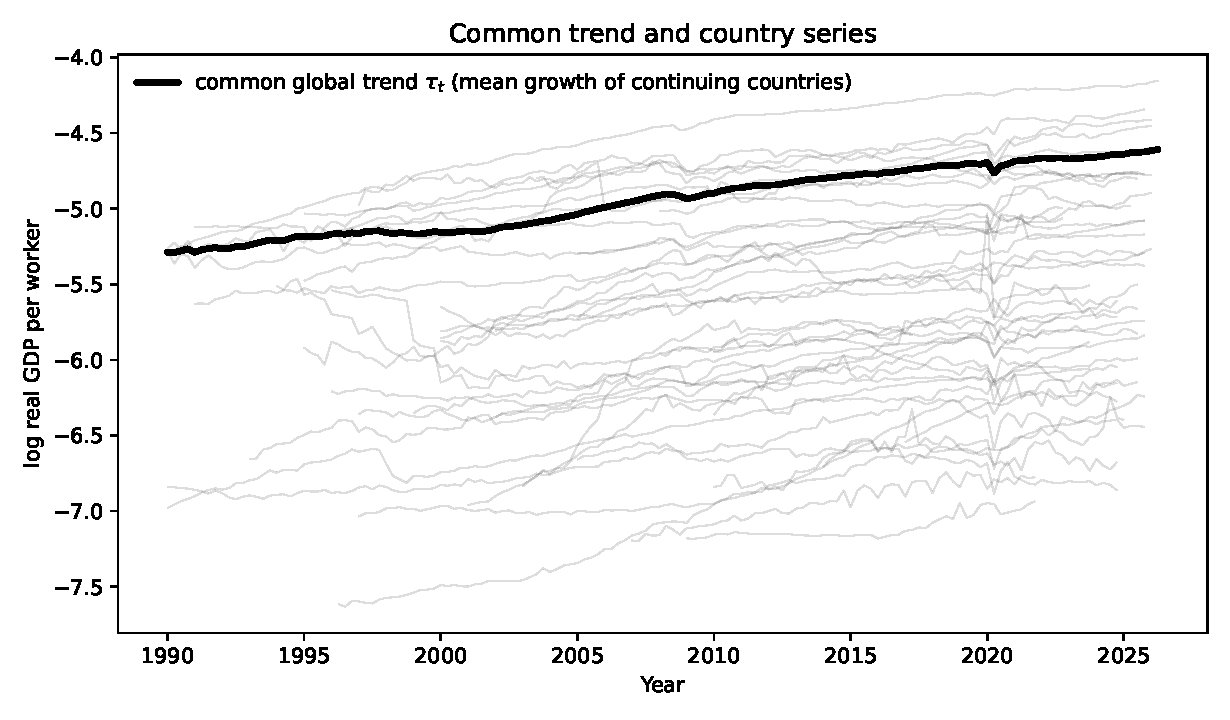
\includegraphics[width=0.88\textwidth]{figs/tau_embi_1990.pdf}
\caption{Faint lines: country log real GDP per worker. Thick line: common $\tau_t$.}
\end{figure}
\clearpage
\section{EMBI countries from 1990: RE intercepts around a common RW trend}
EMBI countries, 1990 onward, $y_{it}=a_i+\tau_t+z_{it}$, $E[z]=0$. 43 countries, 4275 observations, 1990-Q1--2026-Q2. Fitted countries: 43. Observations: 4275. Log-likelihood: 10528.30.
Random intercepts $a_i\sim N(\alpha,\omega^2)$ with $\alpha=-0.7740$ (0.0430), $\omega=0.4470$ (0.0159). Posterior-mean $a_i$: mean -0.872, min -2.514, max 0.507.
\begin{table}[h]
\centering
\caption{Regime AR(1), transition matrix, and ergodic $\pi$. Columns are regimes.}
\begin{tabular}{lccc}
\toprule
 & (0) & (1) & (2) \\
\midrule
$\mu$ & -0.0786 & -0.0400 & 0.0813 \\
 & (0.0746) & --- & (0.0509) \\ \addlinespace
$\sigma$ & 0.0243 & 0.0930 & 0.0095 \\
 & (0.0010) & (0.0058) & (0.0003) \\ \addlinespace
$\rho$ & 0.9900 & 0.9900 & 0.9896 \\
 & (0.0000) & (0.0001) & (0.0012) \\ \addlinespace
$\Pi_{0\cdot}$ & 0.8962 & 0.0378 & 0.0660 \\
 & (0.0152) & (0.0100) & (0.0129) \\ \addlinespace
$\Pi_{1\cdot}$ & 0.2946 & 0.6755 & 0.0299 \\
 & (0.0611) & (0.0593) & (0.0222) \\ \addlinespace
$\Pi_{2\cdot}$ & 0.0600 & 0.0101 & 0.9298 \\
 & (0.0108) & (0.0053) & (0.0098) \\ \addlinespace
$\pi$ & 0.4649 & 0.0688 & 0.4663 \\
 & (0.0333) & (0.0122) & (0.0372) \\ \addlinespace
\bottomrule
\end{tabular}
\end{table}
\begin{figure}[h]
\centering
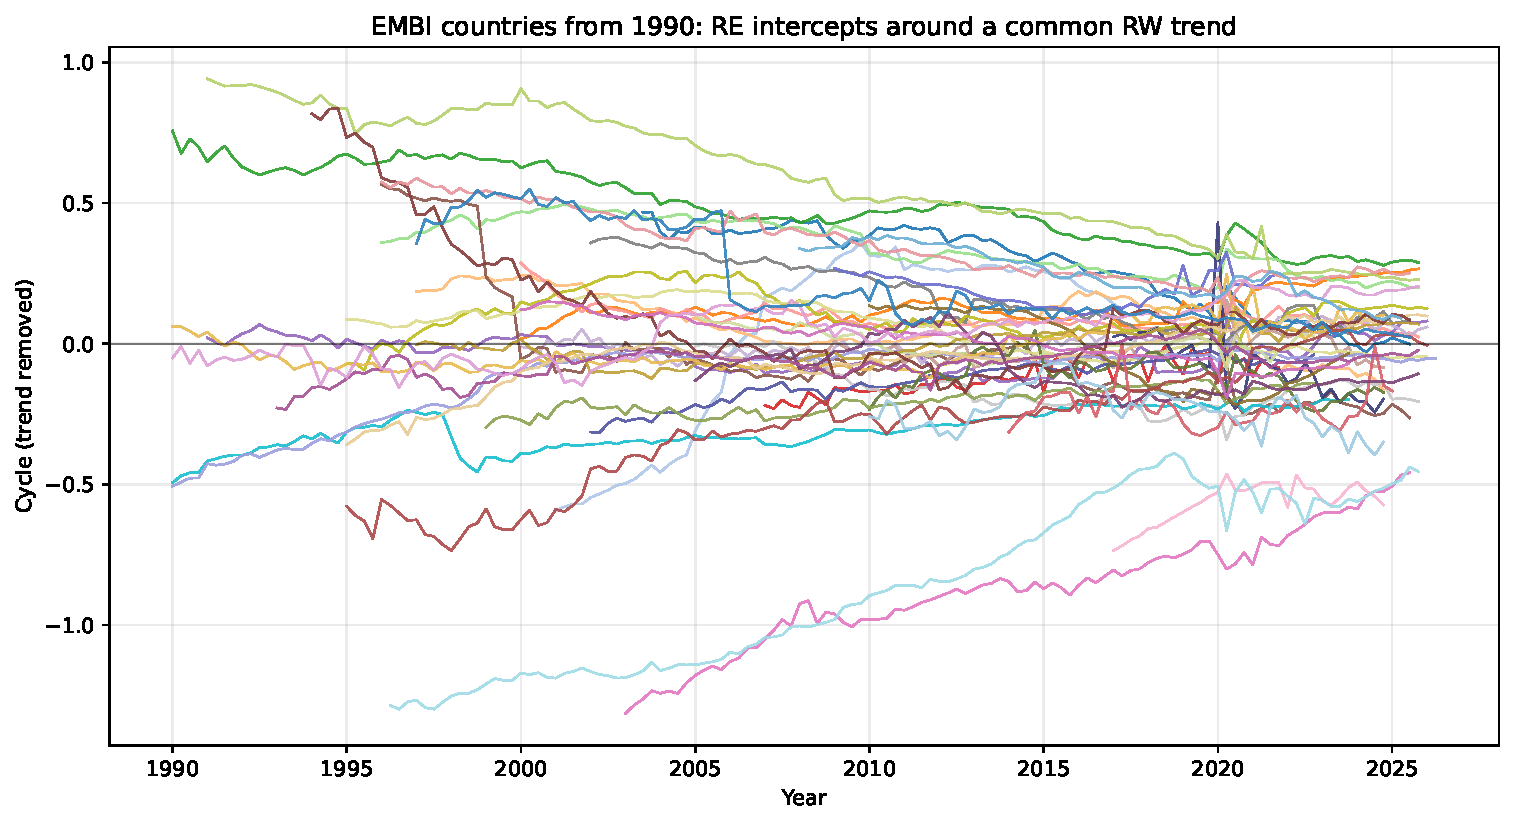
\includegraphics[width=0.75\textwidth]{figs/cycle_embi_1990_rw.pdf}
\caption{Country cycles after removing $\tau_t$ and the posterior-mean intercept.}
\end{figure}
\end{document}
